
Given equation of the parabola is:
\begin{align}
    y^2=8x\\
    y^2-8x=0\\
    y^2+2(-4)=0
\end{align}
comparing it with standard equation
\begin{align}
    ax^2+2bxy+cy^2+2dx+2ey+f=0
\end{align}
$\therefore$  a = b = e = 0, d = -4, c = 1, f = 0
\begin{align}
   \vec{V}=\myvec{a&b\\b&c}=\myvec{0&0\\0&1}\\
   \vec{u}=\myvec{-4\\0} 
\end{align}
\begin{lemma}
The equation of a parabola is:
\begin{align}
    \vec{x}^T\vec{V}\vec{x}+2\vec{u}^T\vec{x}+f=0
\end{align}
Then its vertex can be calculated as :
\begin{align}
    \myvec{\vec{u}^T+\eta\vec{p_1}^T\\\vec{V}}\vec{c}=\myvec{\vec{-f}\\\eta\vec{p_1}-\vec{u}}\\
    \text{where, } \eta=\vec{u^T}\vec{p_1}
\end{align}
\end{lemma}
Equation of the parabola can be written as
\begin{align}
   \implies \myvec{0&0\\0&1}\vec{x}+2\myvec{-4&0}\vec{x}+0=0
\end{align}
We can find the eigen values corresponding to the $\vec{V}$,
\begin{align}
\left|\vec{V}-\lambda\vec{I}\right| =\left|\myvec{0-\lambda&0\\0&1-\lambda}\right|
\end{align}
\begin{align}
    \brak{-\lambda}\brak{1-\lambda}=0
\end{align}
$\therefore$
Eigen values are $ \lambda_1=0,\lambda_2=1$
\\
Calculating the eigen vectors corresponding to  $ \lambda_1=0,\lambda_2=1$ respectively
\begin{align}
    \vec{V}\vec{x}=\lambda\vec{x}
\end{align}
\begin{align}
   \implies \vec{p_1}=\myvec{1\\0}\\
   \implies \vec{p_2}=\myvec{0\\1}
\end{align}
The vertex of the parabola can be given as
\begin{align}
    \myvec{\vec{u}^T+\eta\vec{p_1}^T\\\vec{V}}\vec{c}=\myvec{\vec{-f}\\\eta\vec{p_1}-\vec{u}}\\
   \text{where, } \eta=\vec{u^T}\vec{p_1}=\myvec{-4&0}\myvec{1\\0}
    \end{align}
\begin{align}
    \myvec{-8&1\\0&0\\0&1}\vec{c}=\myvec{0\\0\\0}\\
    \implies \vec{c}=\myvec{0\\0}
\end{align}
Since $\lambda_2 > \lambda_1$\\
Hence, the axis using $\vec{p_2}$ is given by
\begin{align}
    \vec{p_2}^T\myvec{\vec{x}-\vec{c}}=0
    \end{align}
    \begin{align}
     \myvec{0&1}\myvec{x\\y}=0   
    \end{align}
    \begin{align}
       \implies y=0 
    \end{align}
    \begin{align}
    \myvec{0&1}\vec{x}=0
\end{align}
\begin{theorem}
The eccentricity, directrices and foci of parabola are given by\\ 
\text{Eccentricity,}
\begin{align}
    e&= \sqrt{1-\frac{\lambda_1}{\lambda_2}} \label{oct/2/24/eq:1}
\end{align}
\begin{align}
  \vec{n}&= \sqrt{\lambda_2}\vec{p}_1 \label{oct/2/24/eq:2}
  \end{align}
  \begin{align}
  c = \frac{\norm{\vec{u}}^2 - \lambda_2 f   }{2e^2\vec{u}^{\top}\vec{n}} \label{oct/2/24/eq:3}
  \end{align}
 \text{Focus,} 
 \begin{align}
  \vec{F}  &= \frac{ce^2\vec{n}-\vec{u}}{\lambda_2}\label{oct/2/24/eq:4}
\end{align}
\text{Directrix,}
\begin{align}
\vec{n}^T \vec{x}=c \label{oct/2/24/eq:5}
 \end{align}
\end{theorem}
From Equation \ref{oct/2/24/eq:1}, eccentricity can be calculated as
\begin{align}
    e&= \sqrt{1-\frac{\lambda_1}{\lambda_2}}
\end{align}
\begin{align}
    e&= \sqrt{1-\frac{0}{1}} =\sqrt{1}\\
     \implies e&= 1
\end{align}
Substituting $\lambda_2$ and $\vec{p_1}$ values in Equation {\ref{oct/2/24/eq:2}}
\begin{align}
   \vec{n}&= \sqrt{\lambda_2}\vec{p}_1\\
   \vec{n}&= \sqrt{1}\myvec{1\\0}\\
   \implies \vec{n}&=\myvec{1\\0}
\end{align}
Equation \ref{oct/2/24/eq:3} can be calculated as
\begin{align}
    c = \frac{\norm{\vec{u}}^2 - \lambda_2 f   }{2e^2\vec{u}^{\top}\vec{n}}
\end{align}
\begin{align}
    c = \frac{16-1\times0}{2 \times 1^2 \times \myvec{-4&0}\myvec{1\\0}}
\end{align}
\begin{align}
    =\frac{16}{-8}\\
    \implies c = -2
\end{align}
Focus of the parabolic equation can be calculated from the equation \ref{oct/2/24/eq:4} 
 \begin{align}
  \vec{F}  &= \frac{ce^2\vec{n}-\vec{u}}{\lambda_2}
\end{align}
 \begin{align}
  \vec{F}  &= \frac{-2 \times 1 \times \myvec{1\\0}-\myvec{-4\\0}}{1}
\end{align}
\begin{align}
   \implies \vec{F}=\myvec{2\\0} 
\end{align}
Directrix of the parabolic equation can be calculated from equation \ref{oct/2/24/eq:5}
\begin{align}
   \vec{n}^T \vec{x}=c 
\end{align}
\begin{align}
    \myvec{1&0}\vec{x}=-2
\end{align}
Latus rectum is the line which is parallel to the directrix, passes through the focus and four times of the focal length. Since, the focal length of the parabola is 2.\\
$\therefore$ Latus rectum is 8\\
Equation of the latus rectum is
\begin{align}
    \myvec{1&0}\vec{x}=2
\end{align}
\numberwithin{figure}{section}
\begin{figure}[ht]
    \centering
    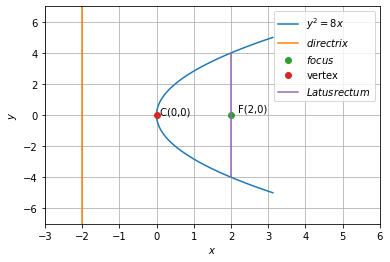
\includegraphics[width=\columnwidth]{solutions/oct/2/24/Graph.png}
    \caption{Parabola}
    \label{oct/2/24/Graphical solution}
\end{figure}
